\documentclass[handout]{beamer}
\usepackage{pgfpages}
\pgfpagesuselayout{2 on 1}[a4paper,border shrink=5mm]
\usepackage{amsmath,amssymb,amsthm,array}
\usepackage{bm}
\usepackage{multirow}
\usepackage{multicol}
\usepackage{algorithm}
\usepackage{hyperref}
\usepackage{algorithmic}
\usepackage[normalem]{ulem}
\usepackage{fontspec}
 

\setmainfont{CMU Serif}
\setsansfont{CMU Sans Serif}
\newfontfamily{\greekfont}{CMU Serif}
\newfontfamily{\greekfontsf}{CMU Sans Serif}


\usetheme{Rochester}
\usecolortheme{beaver}
 

\setbeamertemplate{navigation symbols}{}
\title{Μοντέλα και Αποδείξεις Ασφάλειας στην Κρυπτογραφία - Ανταλλαγή Κλειδιού Diffie Hellman}
\author{Παναγιώτης Γροντάς - Άρης Παγουρτζής}
\date{07/11/2017}
\defbeamertemplate*{footline}{shadow theme}
{%
  \leavevmode%
  \hbox{
		\begin{beamercolorbox}[wd=.4\paperwidth,ht=2.5ex,dp=1.125ex,leftskip=.3cm,rightskip=.3cm plus1fil]{title in head/foot}%
			\usebeamerfont{title in head/foot} Formal Models - DHKE  %
		\end{beamercolorbox}
		\begin{beamercolorbox}[wd=.5\paperwidth,ht=2.5ex,dp=1.125ex,leftskip=.3cm,rightskip=.3cm plus1fil]{title in head/foot}%
			\usebeamerfont{title in head/foot} \hfill \insertsection  %
		\end{beamercolorbox}
		\begin{beamercolorbox}[wd=.1\paperwidth,ht=2.5ex,dp=1.125ex,leftskip=.3cm plus1fil,rightskip=.3cm]{author in head/foot}%
			\usebeamerfont{author in head/foot}\insertframenumber\,/\,\inserttotalframenumber
		\end{beamercolorbox}%
  }%
  \vskip0pt%
}
\institute{ΕΜΠ - Κρυπτογραφία (2017-2018)}


\setlength{\columnseprule}{0.4pt}
\begin{document}

\newcommand{\MSG}{ \mathtt{M} }
\newcommand{\KEY}{ \mathtt{K} }
\newcommand{\CPH}{ \mathtt{C} }
\newcommand{\keygen}{\mathtt{KeyGen}}
\newcommand{\enc}{\mathtt{Encrypt}}
\newcommand{\dec}{\mathtt{Decrypt}}
\newcommand{\adv}{$\mathcal{A} \,$ }
\newcommand{\advb}{$\mathcal{B} \,$ }
\newcommand{\chal}{$\mathcal{C} \,$ }
\newcommand{\cs}{$\mathcal{CS} \,$ }

\newcommand{\green}[1]{\textcolor{teal}{#1}}
\newcommand{\Green}[1]{\textcolor{Teal}{#1}}
\newcommand{\ForestGreen}[1]{\textcolor{ForestGreen}{#1}}
\newcommand{\blue}[1]{\textcolor{blue}{#1}}
\newcommand{\magenta}[1]{\textcolor{magenta}{#1}}
\newcommand{\cyan}[1]{\textcolor{cyan}{#1}}

\newcommand{\twopartdef}[4]
{ 
		\begin{cases}
			#1 , #2 \\
			#3 , #4
		\end{cases} 
}
\begin{frame}
\titlepage
\end{frame}



\begin{frame}{Περιεχόμενα}
\begin{itemize}
\item Ορισμός Κρυπτοσυστήματος
\item Δυνατότητες Αντιπάλου - Επιθέσεις
\item Εμπειρική Ασφάλεια (Kerckhoffs) - Σημασιολογική Ασφάλεια - Μη Διακρισιμότητα
\item Γενική Μορφή Κρυπτογραφικών Αναγωγών
\item Ανταλλαγή Κλειδιού Diffie Hellman
\end{itemize}
\end{frame}

\section{Ορισμοί}
\begin{frame}[allowframebreaks]{Κρυπτοσύστημα} 
\begin{itemize}
\item \cs$=(\MSG, \KEY, \CPH, \keygen, \enc, \dec)$
\item $\MSG$: Σύνολο Μηνυμάτων
\item $\KEY$: Σύνολο Κλειδιών
\item $\CPH$: Σύνολο Κρυπτοκειμένων
\item $\keygen(1^\lambda) = (key_{enc},{key_{dec}}) \in \KEY^2$ 
\begin{itemize}
\item Πιθανοτικός Αλγόριθμος 
\item Το κλειδί συνήθως επιλέγεται \emph{ομοιόμορφα} από το $\KEY$
\item $\lambda:$ Παράμετρος ασφάλειας - πλήθος bits του κλειδιού
\end{itemize}
\item $\enc(key_{enc},m) = c \in \CPH$
\begin{itemize}
\item Ντετερμινιστικός Αλγόριθμος: Κάθε μήνυμα αντιστοιχεί σε ένα κρυπτοκείμενο
\item Πιθανοτικός Αλγόριθμος: Κάθε μήνυμα αντιστοιχεί σε ένα σύνολο πιθανών κρυπτοκειμένων
\end{itemize}
\item $\dec(key_{dec},c) = m$
\end{itemize}
\framebreak
Παρατηρήσεις:
\begin{itemize}
\item Συμμετρικό Κρυπτοσύστημα $key_{enc} = key_{dec}$
\item Ασύμμετρο Κρυπτοσύστημα $key_{enc} \neq key_{dec}$
\begin{itemize}
\item Κρυπτογραφία Δημοσίου Κλειδιού
\item Το $key_{enc}$ μπορεί να δημοσιοποιηθεί για την εύκολη ανταλλαγή μηνυμάτων
\end{itemize}
\item Ορθότητα σε κάθε περίπτωση: $\dec(key_{dec}, \enc(key_{enc}, m)) = m, \forall m \in \MSG$
\end{itemize}
\end{frame}

\begin{frame}{Ο αντίπαλος \adv}
\begin{itemize}
\item Στόχος: Να \emph{σπάσει} το κρυπτοσύστημα
\item Δηλαδή, με δεδομένο το $c$:
\pause
\begin{itemize}
\item Να μάθει το κλειδί $k$; 
\pause
\begin{itemize}
\item Επίθεση Πυρηνικής Βόμβας
\item Θέλουμε να προστατεύσουμε το μήνυμα
\item $\enc(k,m)=m$ παρέχει ασφάλεια αλλά όχι μυστικότητα
\end{itemize}
\pause
\item Να μάθει ολοκληρο το αρχικό μήνυμα $m$;
\begin{itemize}
\item Αν μάθει το 90\%;
\end{itemize}
\pause
\item Να μάθει κάποια συνάρτηση του $m$;
\begin{itemize}
\item Ναι αλλά ποια;
\end{itemize}
\end{itemize}
\pause
\item Συμπέρασμα:Χρειάζονται ακριβείς ορισμοί
\begin{itemize}
\item Για το τι σημαίνει 'σπασιμο'
\item Για τις δυνατότητες και τα μέσα του αντιπάλου.
\end{itemize}
\end{itemize}
\end{frame}

\begin{frame}[allowframebreaks]{Δυνατότητες και Μέσα (Ιστορικά)}
Επιθέσεις
\begin{itemize}
\item Επίθεση Μόνο Κρυπτοκειμένου - Ciphertext Only Attack (COA)
\begin{itemize}
\item Παθητικός Αντίπαλος
\item Πολύ εύκολη: Χρειάζεται απλά πρόσβαση στο κανάλι επικοινωνίας
\end{itemize}
\framebreak
\item Επίθεση Γνωστού Μηνύματος -  Known Plaintext Attack (KPA)
\begin{itemize}
\item Παθητικός Αντίπαλος
\item \magenta{Γνωρίζει ζεύγη μηνυμάτων - κρυπτοκειμένων}
\item Ρεαλιστικό σενάριο για συμμετρικά
\begin{itemize}
\item Ακόμα και τα απόρρητα πρωτόκολλα περιέχουν μη απόρρητα μηνύματα (handshakes, ack)
\item Enigma: Κρυπτοκείμενα πρόγνωσης καιρού
\item Κρυπτογραφημένα μηνύματα γίνονται κάποια στιγμή διαθέσιμα
\end{itemize} 
\pause
\item Τετριμμένο σενάριο για ασύμμετρα
\begin{itemize}
\item O \adv έχει το δημόσιο κλειδί
\item Μπορεί να κατασκευάσει μόνος του όσα ζεύγη θέλει
\end{itemize}
\end{itemize}
\framebreak

Επίθεση Επιλεγμένου Μηνύματος - Chosen Plaintext Attack (CPA)
\begin{columns}

\begin{column}{0.65\textwidth}
\begin{itemize}
\item \magenta{Ενεργός} Αντίπαλος
\item Γνωρίζει ζεύγη μηνυμάτων - κρυπτοκειμένων
\pause  
\item \magenta{Μπορεί να ζητήσει την κρυπτογράφηση μηνυμάτων της επιλογής του (Μαντείο Κρυπτογράφησης)}
\item Ιστορικό Παράδειγμα: Η ναυμαχία του Midway (1942)
\begin{itemize}
\item Αποστολή Πλαστών Μηνυμάτων Με Την Λέξη 'Midway'
\item Συλλογή Επικοινωνιών Με Κρυπτοκείμενα 'AF'
\item Συσχέτιση με παλιότερες επικοινωνίες
\end{itemize}
\end{itemize}
\end{column}

\begin{column}{0.35\textwidth}
\begin{figure} 
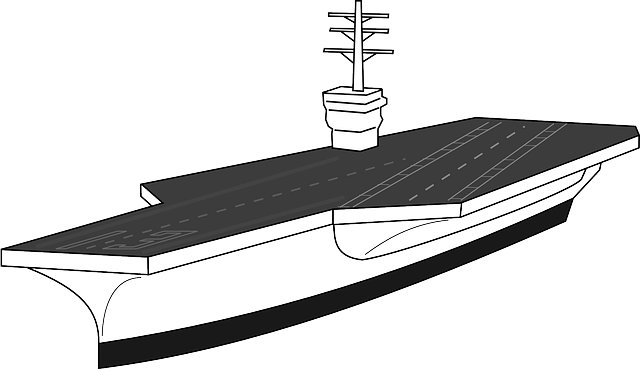
\includegraphics[scale=0.15]{planecarrier.png}  
\end{figure}
\end{column}

\end{columns}

\framebreak

\item Επίθεση Επιλεγμένου Κρυπτοκειμένου - Chosen Ciphertext Attack (CCA)
\begin{itemize}
\item Ενεργός Αντίπαλος
\item Γνωρίζει ζεύγη μηνυμάτων - κρυπτοκειμένων
\item Μπορεί να ζητήσει την κρυπτογράφηση μηνυμάτων της επιλογής του (Μαντείο Κρυπτογράφησης)
\item \magenta{Μπορεί να επιτύχει την αποκρυπτογράφηση μηνυμάτων της επιλογής του (Μαντείο Αποκρυπτογράφησης)}
\item Ο αντίπαλος μπορεί να βγάλει \emph{έμμεσα} συμπεράσματα από αντιδράσεις σε κρυπτογραφημένα μηνύματα
\begin{itemize}
\item Απόρριψη κρυπτογραφημένων 'σκουπιδιών' από το πρωτόκολλο (Bleichenbacher RSA PKCS1 attack)
\item Ενέργεια στον πραγματικό κόσμο (πχ. αγορά μετοχών)
\end{itemize}
\end{itemize}
\end{itemize}
\end{frame}

\begin{frame}[allowframebreaks]{Οι κανόνες του Kerchoffs (1883)}

Οι πρώτες προσπάθειες ορισμού ασφάλειας κρυπτοσυστήματων και προστασίας 

\begin{block}{Αρχή 2}
Ο αλγόριθμος(από)κρυπτογράφησης δεν πρέπει να είναι μυστικός. Πρέπει να μπορεί να πέσει στα χέρια του \adv χωρίς να δημιουργήσει κανένα πρόβλημα. Αντίθετα το κλειδί μόνο πρέπει να είναι μυστικό.
\end{block}

Λόγοι:
\pause 

\begin{itemize}
\item Tο κλειδί διανέμεται πιο εύκολα από τους αλγόριθμους (μικρότερο μέγεθος, απλούστερη δομή)  
\item Το κλειδί είναι πιο εύκολο να αλλαχθεί αν διαρρεύσει
\item Πιο πρακτική χρήση για περισσότερους από έναν συμμετέχοντες
\item Ανοικτό κρυπτοσύστημα: Εύκολη μελέτη 
\end{itemize}

Παρατηρήσεις:

Αν και έχουν παράδοση ακόμα και σήμερα δεν εφαρμόζονται πλήρως
\begin{itemize}
\item (Μεγάλες) εταιρίες δημιουργούν και χρησιμοποιούν δικούς τους μυστικούς αλγόριθμους/πρωτόκολλα
\begin{itemize}
\item Bruce Schneier \href{https://goo.gl/FaFoSK}{Crypto Snake Oil}
\end{itemize}

\end{itemize}
 

\framebreak
\begin{block}{Αρχή 1}
Το κρυπτοσύστημα θα πρέπει να είναι \emph{πρακτικά} απρόσβλητο, αν δεν γίνεται θεωρητικά
\end{block}
\begin{itemize}
\item Διάρκεια Κρυπτανάλυσης > Διάρκεια Ζωής Μηνύματος
\item Μικρή Πιθανότητα Επιτυχίας
\item Υπολογιστική Ασφάλεια
\end{itemize}
\pause 

Σε κάθε περίπτωση - Εμπειρικές Αρχές: 

Δεν αντιστοιχίζονται σε κάτι απτό
\end{frame}

\section{'Αποδείξιμη' Ασφάλεια}

\begin{frame}{Γενικά}

\begin{block}{Ιδέα}
Μαθηματική (Λογική) απόδειξη ότι το κρυπτοσύστημα έχει κάποιες ιδιότητες ασφάλειας.
\end{block}

Παράδειγμα: Τέλεια μυστικότητα (Shannon)

\magenta{Πρόβλημα}: Μπορεί να εφαρμοστεί στην κρυπτογραφία δημοσίου κλειδιού; Γιατί;

\pause 

Επαναχρησιμοποίηση δημοσίου κλειδιού

\end{frame}

\begin{frame}[allowframebreaks]{Σημασιολογική Ασφάλεια}
Βασική ιδέα (Goldwasser, Micali): Χαλαρώνουμε τις υποθέσεις για να οδηγηθούμε σε έναν πιο χρήσιμο ορισμό, λαμβάνοντας υπόψιν:

\begin{itemize}
	\item την υπολογιστική ισχύ του \adv
	\item την πιθανότητα επιτυχίας
	\item το είδος των επιθέσεων
\end{itemize}

\begin{block}{Διαίσθηση}
Ένας υπολογιστικά περιορισμένος \adv  δεν μπορεί να μάθει τίποτε χρήσιμο από το κρυπτοκείμενο παρά μόνο με αμελητέα πιθανότητα
\end{block}

\framebreak
\begin{block}{Ρητή Προσέγγιση}
Ένα κρυπτοσύστημα είναι $(\tau,\epsilon)$ ασφαλές αν οποιοσδήποτε \adv σε χρόνο το πολύ $\tau$, δεν μπορεί να το σπάσει με πιθανότητα καλύτερη από $\epsilon$ 
\end{block}
Για συμμετρικά κρυπτοσυστήματα σήμερα $\tau=2^{80}$ και $\epsilon=2^{-64}$

\alert{Δεν χρησιμοποιείται} γιατί

\begin{itemize}
\item Δεν ασχολείται με το υπολογιστικό μοντέλο (κατανεμημένοι υπολογιστές, εξειδικευμένο HW κτλ.)
\item Δεν ασχολείται με το τι θα γίνει μετά το $\tau$
\item Για τους ίδιους λόγους με Υπολογιστική Πολυπλοκότητα
\end{itemize}

\framebreak

\begin{block}{Ασυμπτωτική Προσέγγιση}
Ένα κρυπτοσύστημα είναι ασφαλές αν οποιοσδήποτε PPT \adv έχει αμελητέα πιθανότητα να το σπάσει (σε σχέση με την παράμετρο ασφάλειας)
\end{block}

Παρατηρήσεις:
\begin{itemize}
\item Ισχύει για μεγάλες τιμές του $\lambda$
\item Συνέπεια του $|\KEY| < |\MSG|$
\item Επιτρέπει προσαρμογή της ασφάλειας με αλλαγή του μήκους του κλειδιού
\end{itemize}
 
\framebreak

Τυπικός Ορισμός: Υποθέσεις
\begin{itemize}
\item O \adv θέλει να υπολογίσει το κατηγόρημα $q: \MSG \rightarrow \{0,1\}$
\item $Pr_{m \in \MSG}[q(m)=0]=Pr_{m \in \MSG}[q(m)=1]=\frac{1}{2}$
\item Το μήκος των κρυπτοκειμένων είναι το ίδιο (δεν διαρρέει πληροφορία)
\end{itemize}

\begin{block}{Το πλεονέκτημα του \adv}
$Adv(\mathcal{A}) = |Pr[\mathcal{A}(c)=q(\dec(key,c))]-\frac{1}{2}|$
\end{block}

Παρατήρηση: Αν ο \adv μαντέψει στην τύχη έχει $Adv(\mathcal{A})=0$
\framebreak

\begin{block}{Ορισμός}
Ένα κρυπτοσύστημα είναι σημασιολογικά ασφαλές όταν $\forall$ PPT \adv, $\forall q$:
\begin{center}
$Adv(\mathcal{A})=negl(\lambda)$
\end{center}
\end{block}

Αμελητέα συνάρτηση: Μεγαλώνει με πιο αργό ρυθμό από αντίστροφο πολυώνυμο

\framebreak

\begin{block}{Αμελητέα συνάρτηση}
Οποιαδήποτε συνάρτηση για την οποία για κάθε πολυώνυμο $p$ υπάρχει $n_0$ ώστε $\forall n \geq n_0: neql(n)<\frac{1}{p(n)}$
\end{block}

Συνήθως: $c2^{-n},2^{-\sqrt{n}},n^{-log{n}} $
 
\begin{block}{Παρατηρήσεις}
\begin{itemize}
\item Ο τυπικός ορισμός ενσωματώνει την παράμετρο ασφαλείας
\item Δύσχρηστος ορισμός
\item Δεν ορίσαμε ακριβώς τη διαδικασία προς το 'σπάσιμο'
\end{itemize}
\end{block}
\end{frame}

\begin{frame}[allowframebreaks]{Μη Διακρισιμότητα(Indistinguishability)}
Παίγνιο Μη Διακρισιμότητας μεταξύ των \adv, \chal (αναπαριστά το κρυπτοσύστημα)
\begin{columns}
\begin{column}{0.4\textwidth}
\begin{itemize}
\item Ανταλλαγή Μηνυμάτων μεταξύ \adv, \chal
\item \adv: Παράγει δύο μηνύματα $m_0, m_1$
\item \chal: Διαλέγει ένα τυχαίο bit $b$
\item \chal: Παράγει και απαντά με το $c_b = \enc(m_b)$
\item \adv: Μαντεύει ένα bit $b'$
\end{itemize}
\end{column}
\begin{column}{0.6\textwidth}
\begin{figure} 
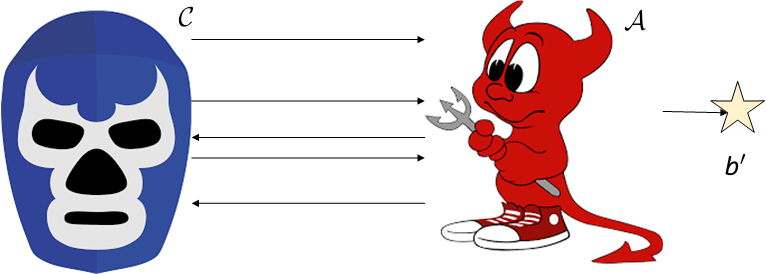
\includegraphics[scale=0.3]{game.png}  
\end{figure}

$IND-Game(\mathcal{A}) = \twopartdef{1}{b'=b}{0}{\text{αλλιώς}}$

\end{column}
\end{columns}

\framebreak

\begin{block}{Πλεονέκτημα}
$Adv_{IND}(\mathcal{A}) = |Pr[IND-Game(\mathcal{A})=1]-\frac{1}{2}|$
\end{block}

\begin{block}{Ορισμός}
Ένα κρυπτοσύστημα  διαθέτει την ιδιότητα της μη διακρισιμότητας όταν $\forall$ PPT \adv:
\begin{center}
$Adv_{IND}(\mathcal{A}) =negl(\lambda)$
\end{center}
\end{block}

\begin{block}{Θεώρημα}
Σημασιολογική Ασφάλεια $\Leftrightarrow$ Μη-Διακρισιμοτητα
\end{block}

\end{frame}

\section{Μοντελοποίηση Επιθέσεων}
\begin{frame}{IND-EAV}
\begin{figure} 
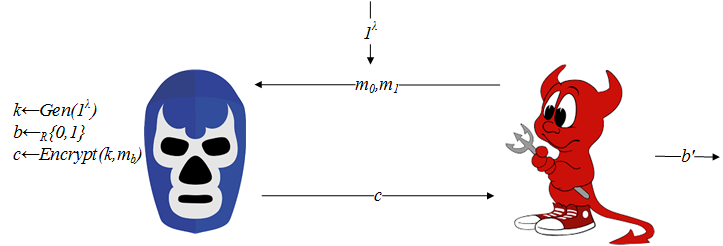
\includegraphics[scale=0.6]{ind-eav.png}  
\end{figure}
\end{frame}

\begin{frame}{IND-CPA}
\begin{figure} 
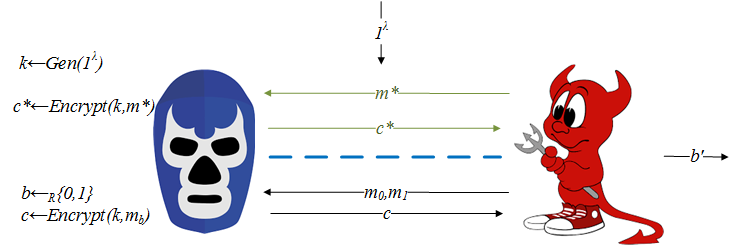
\includegraphics[scale=0.6]{ind-cpa.png}  
\end{figure}
\end{frame}

\begin{frame}{Παρατηρήσεις}
\begin{block}{Θεώρημα}
Ένα κρυπτοσύστημα με ντετερμινιστικό αλγόριθμο κρυπτογράφησης δεν μπορεί να έχει την ιδιότητα IND-CPA.
\end{block}
{Απόδειξη}
\pause

\begin{itemize}
\item O \adv θέτει $m^*=m_0$ και λαμβάνει την κρυπτογράφηση $c^*$
\item Η απάντηση του είναι $b'=\twopartdef{0}{c^*=c}{1}{\text{αλλιώς}}$
\item O \adv κερδίζει πάντα $Pr[IND-CPA(\mathcal{A})=1]=1$
\end{itemize}

\end{frame}
\begin{frame}{IND-CCA}
\begin{figure} 
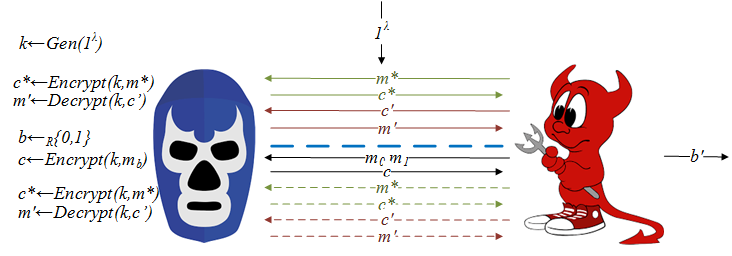
\includegraphics[scale=0.6]{ind-cca.png}  
\end{figure}
\end{frame}

\begin{frame}{Παρατηρήσεις}
\begin{itemize}
\item Στο παίγνιο IND-CCA o \adv δεν μπορεί να ρωτήσει τον $C$ για την αποκρυπτογραφήση του $c$
\item Μπορεί όμως να:
\begin{itemize}
\item Μετατρέψει το $c$ σε $\hat{c}$
\item Ζητήσει την αποκρυπτογράφηση του $\hat{c}$ σε $\hat{m}$
\item Να μετατρέψει το $\hat{m}$ σε $m$, κερδίζοντας με πιθανότητα 1
\end{itemize}
\pause
\item IND-CCA2: Επιτρέπεται χρήση του μαντείου αποκρυπτογράφησης μετά το $c$ (adaptive IND-CCA)
\item IND-CCA1: αλλιώς
\end{itemize}
\end{frame}

\begin{frame}[allowframebreaks]{Malleability}

\begin{block}{\emph{Malleable (εύπλαστο)} Κρυπτοσύστημα}
Επιτρέπει στο \adv να φτιάξει, γνωρίζοντας μόνο το κρυπτοκείμενο $c=\enc(m)$, ένα \emph{έγκυρο} κρυπτοκείμενο $c'=\enc(h(m))$, για κάποια, συνήθως πολυωνυμικά αντιστρέψιμη, συνάρτηση $h$ γνωστή σε αυτόν. 
\end{block}
 

\begin{block}{Σημαντική ιδιότητα}
Non-malleability $\Leftrightarrow$ IND-CCA2
\end{block}

\framebreak

Κάποιες φορές είναι επιθυμητή και κάποιες όχι.
\begin{itemize}
\item Ομομορφικά Κρυπτοσυστήματα: Αποτίμηση μερικών πράξεων στα κρυπτοκείμενα (ηλ. ψηφοφορίες)
\item Πλήρως Ομομορφικά Κρυπτοσυστήμα (Gentry 2010): Αποτίμηση οποιουδήποτε κυκλώματος στα κρυπτοκείμενα
\item Δεν μπορούν να είναι IND-CCA2, ... αλλά είναι πολύ χρήσιμα
\end{itemize}
 
 
\end{frame}

\section{Αναγωγή}
\begin{frame}[allowframebreaks]{Κρυπτογραφικές Αναγωγές}
\begin{block}{Γενική Μορφή}
Αν ισχύει η υπόθεση $\mathcal{Y}$, τότε και το κρυπτοσύστημα \cs είναι ασφαλές (υπό συγκεκριμένο ορισμό).
\end{block}
\medskip

\begin{block}{Αντιθετοαντιστροφή}
Αν το \cs ΔΕΝ είναι ασφαλές (υπό συγκεκριμένο ορισμό), τότε δεν ισχύει η $\mathcal{Y}$.
\end{block}

Κατασκευαστική απόδειξη

\framebreak

\begin{itemize}
\item \cs μη ασφαλές $\Rightarrow$ $\exists$ PPT \adv  o οποίος παραβιάζει τον ορισμό ασφάλειας
\item \emph{Κατασκευάζουμε} PPT αλγόριθμο  $\mathcal{B}$, ο οποίος αλληλεπιδρά με τον $\mathcal{C}_y$ ο οποίος προσπαθεί να 'υπερασπιστεί' την $\mathcal{Y}$
\item Ο $\mathcal{B}$ για να καταρρίψει την $\mathcal{Y}$ χρησιμοποιεί εσωτερικά σαν υπορουτίνα τον \adv (black box access) παριστάνωντας τον $\mathcal{C}$ στο παίγνιο μη διακρισιμότητας του \cs
\end{itemize}

\framebreak

\begin{figure}
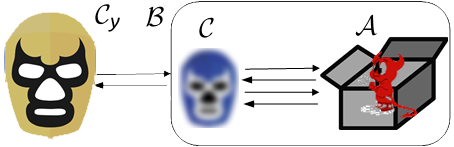
\includegraphics[scale=0.8]{ProofReduction.png}  
\end{figure}
 
\end{frame}

\begin{frame}{Παρατηρήσεις}
Κανόνες Ορθότητας
\begin{itemize}
	\item Προσομοίωση: Ο \adv δεν θα πρέπει να ξεχωρίζει τον $\mathcal{B}$ από οποιονδήποτε άλλο εισηγητή.
	\item Πιθανότητα επιτυχίας: Αν ο \adv έχει μη αμελητέα πιθανότητα επιτυχίας τότε και ο $\mathcal{B}$ θα πρέπει να έχει μη αμελητέα πιθανότητα
	\item Πολυπλοκότητα: Ο $\mathcal{B}$ θα πρέπει να είναι PPT. Αυτό πρακτικά σημαίνει ότι όποια επιπλέον εσωτερική επεξεργασία  πρέπει να είναι πολυωνυμική  
	\item Πρέπει να είναι όσο πιο tight γίνεται ($t_\mathcal{B} \approx t_\mathcal{A}$ και $\epsilon_\mathcal{B} \approx \epsilon_\mathcal{A}$)
\end{itemize}
\end{frame}

\begin{frame}{Συμπεράσματα-Συζήτηση}
Κρυπτογραφικές Αναγωγές
\begin{itemize}
\item Παρέχουν σχετικές εγγυήσεις (Δύσκολο Πρόβλημα, Μοντέλο Ασφάλειας)
\item Δίνουν ευκαιρία να ορίσουμε καλύτερα το κρυπτοσύστημα/πρωτόκολλο
\item Πρακτική Χρησιμότητα: Ρύθμιση Παραμέτρου Ασφάλειας
\item Συγκέντρωση Κρυπταναλυτικών Προσπαθειών στο Πρόβλημα Αναγωγής και όχι σε κάθε κρυπτοσύστημα ξεχωριστά
\item Πιο σημαντικές όσο πιο πολύπλοκο γίνεται το πρωτόκολλο
\item Αποδεικνύουν την ασφάλεια του μοντέλου
\begin{itemize}
	\item Πόσο αναπαριστά το μοντέλο την πραγματικόητα; #KRACK
	\item Δεν σημαίνει ότι οποιαδήποτε υλοποίηση θα είναι ασφαλής
\end{itemize}
\end{itemize}
\end{frame}\section{Ανταλλαγή Κλειδιού Diffie Hellman}
\begin{frame}{Το πρωτόκολλο DHKE}
\begin{center}
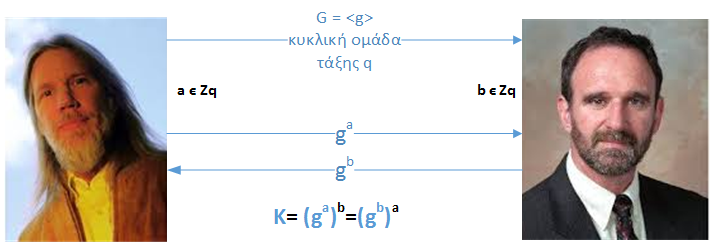
\includegraphics[scale=0.55]{dh.png}
\end{center} 
\pause
Πρωτόκολλο \textbf{Δημιουργίας} Κλειδιού \\
\pause
\textbf{Απαιτήσεις}: \\
Ορθότητα: Αντιμεταθετική ιδιότητα \\
Ασφάλεια: Ύψωση σε δύναμη - μονόδρομη συνάρτηση στην $\mathbb{G}$
\pause 
Συνήθως: $\mathbb{G}$ υποομάδα του $\mathbb{Z}_p^*$ με $p$ πρώτο\\
\pause
Εφαρμογές: SSL, TLS, IPSEC
\end{frame}

\begin{frame}[allowframebreaks]{Σχετιζόμενα Προβλήματα}

\begin{block}{DLP - Το πρόβλημα του Διακριτού Λογαρίθμου}
Δίνεται μια κυκλική ομάδα $\mathbb{G}=<g>$ τάξης $q$ και ένα τυχαίο στοιχείο $y \in \mathbb{G}$

Να υπολογιστεί $x \in \mathbb{Z}_q$ ώστε $g^x = y$ \\
δηλ. το $log_g y \in \mathbb{Z}_q$
\end{block}

\magenta{Αγνοούμε δεδομένα στο πρωτόκολλο DHKE}
\framebreak

\begin{block}{CDHP - Το υπολογιστικό πρόβλημα Diffie Hellman}
Δίνεται μια κυκλική ομάδα $\mathbb{G}=<g>$, δύο στοιχεία $y_1=g^{x_1}, y_2 = g^{x_2}$

Να υπολογιστεί το $g^{x_1 \cdot x_2}$ 
\end{block}


\framebreak
\green{Μπορούμε να δοκιμάζουμε τυχαία στοιχεία}

\begin{block}{DDHP - Το πρόβλημα απόφασης Diffie Hellman}
Δίνεται μια κυκλική  ομάδα $\mathbb{G}=<g>$, δύο στοιχεία $y_1=g^{x_1}, y_2 = g^{x_2}$ και κάποιο  $y \in \mathbb{G}$ 

Να εξεταστεί αν  $y = g^{x_1 \cdot x_2}$ 
\end{block}
ή ισοδύναμα
\begin{block}{DDHP - Το πρόβλημα απόφασης Diffie Hellman}
Δίνεται μια κυκλική  ομάδα $\mathbb{G}=<g>$, δύο στοιχεία $y_1=g^{x_1}, y_2 = g^{x_2}$ και κάποιο  $y \in \mathbb{G}$ 

Μπορούμε να ξεχωρίσουμε τις τριάδες ($g^{x_1}, g^{x_2}, g^{x_1x_2}$) και  ($g^{x_1}, g^{x_2}, y$);
\end{block}
\end{frame}

\begin{frame}{Σχέσεις Προβλημάτων}
\begin{block}{$CDHP \leq DLP$}
Αν μπορούμε να λύσουμε το $DLP$, τότε μπορούμε να υπολογίζουμε τα $x_1, x_2$ από τα $y_1, y_2$ και στην συνέχεια το $g^{x_1 \cdot x_2}$
\end{block}

\pause
 
\begin{block}{$DDHP \leq CDHP$}
Αν μπορούμε να λύσουμε το $CDHP$, υπολογίζουμε το $g^{x_1 \cdot x_2}$ και ελέγχουμε ισότητα με το $y$
\end{block}
 
\pause 
Δηλαδή: $DDHP \leq CDHP \leq DLP$

\alert{Δεν γνωρίζουμε αν ισχύει η αντίστροφη σειρά - ισοδυναμία}
\alert{Όμως:}
Υπάρχουν ομάδες όπου το $DDHP$ έχει αποδειχθεί εύκολο, ενώ $CDHP$ δεν έχει αποδειχθεί εύκολο\\
\alert{Μάλλον:} $DDHP < CDHP$
\end{frame}

\begin{frame}[allowframebreaks]{Ασφάλεια DHKE}

\begin{block}{Διαίσθηση}
Ένας (παθητικός) αντίπαλος δεν αποκτά καμία χρήσιμη πληροφορία για το κλειδί που δημιουργείται.\\
\green{Ισοδύναμα}\\
Ένας (παθητικός) αντίπαλος δεν μπορεί να διακρίνει το κλειδί από ένα τυχαίο στοιχείο της ομάδας στην οποία ανήκει
\end{block}

\framebreak

\begin{block}{Παιχνίδι ανταλλαγής κλειδιού $KEG(\lambda,\Pi,\mathcal{A})$}
\begin{itemize}
\item Εκτέλεση πρωτοκόλλου $\Pi(1^\lambda) \rightarrow (\tau,k)$
\item $\tau$: Τα μηνύματα που ανταλλάσσονται (δημόσια)
\item $k$: Το κλειδί που παράγεται (ιδιωτικό)
\item Επιλογή τυχαίου $b \in \{0,1\}$
\item Αν $b = 0$ επιλογή τυχαίου $k'$ αλλιώς $k'=k$
\item Εκτέλεση \adv$(\tau,k') \rightarrow b'$
\item Αν $b'\neq b$ τότε το αποτέλεσμα του παιχνιδιού είναι $0$, αλλιώς $1$
\end{itemize}
\end{block}

\framebreak

\begin{block}{Ορισμός ασφάλειας}
Ένα πρωτόκολλο ανταλλαγής κλειδιού $\Pi$ είναι ασφαλές, αν κάθε PPT \emph{παθητικός} αντίπαλος \adv έχει αμελητέα πιθανότητα ως προς την παράμετρο ασφάλειας να επιτύχει στο $KEG$

\medskip
\medskip

\green{$Prob[KEG(\lambda,\Pi,\mathcal{A})=1] \leq \frac{1}{2}+negl(\lambda)$}
\end{block}

\end{frame}

\begin{frame}{Απόδειξη ασφάλειας DHKE}
\begin{block}{$DDH \implies DHKE$}
Αν το DDHP είναι δύσκολο, τότε το πρωτόκολλο DHKE είναι ασφαλές (απέναντι σε παθητικό αντίπαλο).
\end{block}

\pause

\textbf{Απόδειξη - Σχεδιάγραμμα}
\begin{small}
Έστω ότι το DHKE δεν είναι ασφαλές. 

$\exists$\adv ώστε \alert{$Prob[KEG(\lambda,\Pi,\mathcal{A})=1] > \frac{1}{2}+non-negl(\lambda)$}

Θα κατασκευάσουμε αντίπαλο PPT \advb ο οποίος παραβιάζει την $DDH$.
\pause

Τα μηνύματα που ανταλλάσσονται είναι τα  $\tau= (\mathbb{G},g,g^{x_1},g^{x_2})$

Εκτελούμε τον \adv με είσοδο $(\tau,g^{x_1x_2})$
\pause

Επειδή το $g^{x_1x_2}$ είναι έγκυρο κλειδί:

\green{$Prob[KEG(\lambda,\Pi,\mathcal{A}(\tau,g^{x_1x_2}))=1]>\frac{1}{2}+non-negl(\lambda)$} 
\pause

Εκτελούμε τον  \adv με είσοδο  $(\tau,y)$ με $y \in_R \mathbb{G}$

Επειδή το $y$ είναι τυχαίο στοιχείο:

\magenta{$Prob[KEG(\lambda,\Pi,\mathcal{A}$(\tau,y)$)=1]=\frac{1}{2}$}
\pause

Άρα ο \advb μπορεί να σπάσει την DDH γιατί μπορεί να ξεχωρίσει με μη αμελητέα πιθανότητα το $y$ από το $g^{x_1,x_2}$ \pause \alert{ΑΤΟΠΟ}
\end{small}
\end{frame}

\begin{frame}{Ενεργοί Αντίπαλοι}
\alert{Man In The Middle Attacks}
\begin{center}
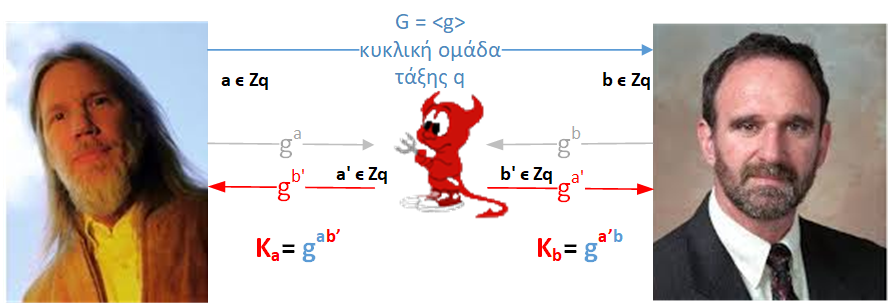
\includegraphics[scale=0.6]{dh-mitm.png}
\end{center} 
\pause
\alert{\href{https://www.schneier.com/blog/archives/2015/02/man-in-the-midd_7.html}{Superfish - Lenovo (02/2015)}}\\
\alert{\href{http://arstechnica.com/security/2015/11/dell-apologizes-for-https-certificate-fiasco-provides-removal-tool/}{DELL - 10/2015}}
\end{frame}


\section{Πηγές}
\begin{frame}[allowframebreaks]{Βιβλιογραφία}
\begin{small}
\begin{itemize}
\item St. Zachos and Aris Pagourtzis. Στοιχεία Θεωρίας Αριθμών και Εφαρμογές στην Κρυπτογραφία. Πανεπιστημιακές Σημειώσεις
\item Jonathan Katz and Yehuda Lindell. Introduction to Modern Cryptography (Chapman and Hall/Crc Cryptography and Network Security Series). Chapman
and Hall/CRC, 2007
\item \href{http://goo.gl/b75I29}{Nigel Smart. Introduction to cryptography} 

\item Alptekin Kupcu. \href{https://goo.gl/l4GT2u}{Proofs In Cryptography}

\item S. Goldwasser and S. Micali. Probabilistic encryption. Journal of Computer and System Sciences, 28(2):270–299, 1984.
\item S. Micali, C. Rackoff, and B. Sloan. The notion of security for probabilistic cryptosystems. SIAM J. Computing, 17(2):412–426, 1988.

\framebreak

\item W. Diffie and M. Hellman. New directions in cryptography. IEEE Trans. Inf. Theor., 22(6):644-654, September 1976

\item Ivan Damgard, \href{http://goo.gl/mgAXC8}{A proof reading of some issues in cryptography}
\item Neil Koblitz, Alfred Menezes \href{https://goo.gl/GJNklR}{Another Look at “Provable Security”}

\item Dan Boneh (1998). "The Decision Diffie–Hellman Problem". ANTS-III: Proceedings of the Third International Symposium on Algorithmic Number Theory. Springer-Verlag: 48–63. doi:10.1007/bfb0054851

\item \href{https://www.schneier.com/}{Bruce Schneier's Blog}
\begin{itemize}
\item \href{https://goo.gl/92TW36}{Memo to the Amateur Cipher Designer} (\url{https://goo.gl/92TW36})
\item \href{https://goo.gl/FaFoSK}{Crypto Snake Oil} (\url{https://goo.gl/FaFoSK})
\end{itemize}
\item \href{http://blog.cryptographyengineering.com/}{A Few Thoughts on Cryptographic Engineering}
\item \href{http://goo.gl/whmmb9}{Bristol Cryptography Blog}

\item \href{https://goo.gl/SHnu8K}{Kerckhoffs Wikipedia Entry} (\url{https://goo.gl/SHnu8K})



\end{itemize}
\end{small}
\end{frame}

 
\end{document}
